\documentclass[conference]{IEEEtran}
\IEEEoverridecommandlockouts

\usepackage{cite}
\usepackage{amsmath,amssymb,amsfonts}
\usepackage{algorithmic}
\usepackage{graphicx}
\usepackage{textcomp}
\usepackage{xcolor}
\usepackage{booktabs}
\usepackage{tabularx}
\usepackage{url}

\def\BibTeX{{\rm B\kern-.05em{\sc i\kern-.025em b}\kern-.08em
    T\kern-.1667em\lower.7ex\hbox{E}\kern-.125emX}}

\renewenvironment{abstract}{%
  \begin{center}%
    \bfseries\large Abstract\par\vspace{0.8ex}%
  \end{center}%
  \bfseries\small\noindent\ignorespaces%
}{%
  \par\vspace{1.5ex}%
}

\renewenvironment{IEEEkeywords}{%
  \par\vspace{0.8ex}\noindent\textbf{\textit{Index Terms:}}\hspace{0.5em}\bfseries\small\ignorespaces%
}{%
  \par\vspace{1.5ex}%
}

\begin{document}

\title{
\noindent\rule{\linewidth}{2.5pt}\vspace{1.5ex}\\
DocSort: A Two-Stage Architecture for Regulatory Document Triage and Verifiable Metadata Extraction\vspace{1.2ex}\\
\noindent\rule{\linewidth}{0.8pt}\vspace{-1ex}
}

\author{
\IEEEauthorblockN{Chinmayi G V}
\IEEEauthorblockA{CSE \\
chinmayi.gv@presidencyuniversity.in}
\and[\hfill\mbox{}\par\vspace{2.5ex}\mbox{}\hfill]
\IEEEauthorblockN{Keerthan Shetty}
\IEEEauthorblockA{CSE \\
keerthans334@gmail.com}
\and
\IEEEauthorblockN{S Mohammed Saheem}
\IEEEauthorblockA{CSE \\
saheemtab@gmail.com}
\and
\IEEEauthorblockN{Tharun H N}
\IEEEauthorblockA{CSE \\
tharun30115@gmail.com}
}

\maketitle

\begin{abstract}
Compliance management in public procurement mandates tracking policy updates and administrative memoranda issued across disparate governmental portals. Manual inspection is labor-intensive and prone to transcription errors, while submitting every incoming document to commercial large language model application programming interfaces incurs high operating expenses, rate-limit starvation, and factual hallucinations. This paper presents DocSort, a two-stage document processing architecture for regulatory document classification and verifiable metadata extraction. In the first stage, a linear classifier utilizing sublinear term-frequency features filters out non-procurement administrative circulars in 3.8 milliseconds on a single central processing unit thread. In the second stage, relevant documents are processed by an instruction-tuned language model under schema constraints and a closed category taxonomy. A deterministic verification component subsequently confirms that extracted factual parameters appear verbatim in the original document text, recording explicit audit flags for discrepancies. To address the lack of domain-specific labeled corpora, a dataset construction method is developed using paragraph-level chunking and weak supervision. Empirical evaluation demonstrates that early linear filtering eliminates 57.0\% of language model invocations, reducing token volume and processing latency by over half while maintaining 0.94 classification F1-score and zero category drift.
\end{abstract}

\begin{IEEEkeywords}
Document classification, public procurement, information extraction, weak supervision, natural language processing.
\end{IEEEkeywords}

\section{Introduction}

Public procurement across government departments and statutory agencies in India is regulated by the General Financial Rules (GFR), directives from the Central Vigilance Commission (CVC), and notifications published by the Department of Expenditure (DoE) under the Ministry of Finance. These regulatory bodies issue Office Memoranda (OMs), amendments, and policy circulars that establish financial thresholds, vendor qualification criteria, mandatory electronic procurement through the Government e-Marketplace (GeM), and contractual penalty clauses.

Compliance officers must examine these circulars continuously to maintain organizational adherence. In current practice, administrative staff manually monitor government web portals, download circulars, and record metadata into spreadsheets. This workflow is slow, demands extensive human effort, and introduces transcription errors on official reference identifiers and statutory effective dates.

Large language models (LLMs) can parse unstructured legal and administrative text. However, deploying monolithic LLM pipelines across incoming document streams introduces operational difficulties. First, government circular streams exhibit pronounced class imbalance: over 80\% of published circulars consist of general administrative notices, such as holiday announcements, employee transfers, and welfare circulars. Submitting all documents to commercial language model endpoints consumes excessive token quotas and causes API rate-limit exhaustion. Second, generative language models frequently hallucinate factual values, generating modified memorandum identifiers and incorrect dates. In formal compliance audits, an ungrounded or fabricated reference identifier invalidates the audit trail.

This paper presents DocSort, a two-stage processing architecture designed for regulatory document triage and verifiable metadata extraction. The pipeline couples a lightweight classical machine learning filter with a constrained generative extraction module and a deterministic verbatim verification layer. The primary contributions are:
\begin{enumerate}
    \item A two-stage pipeline wherein a linear classifier filters non-procurement documents on standard CPU hardware prior to language model invocation, reducing token consumption by 57.0\% and average latency from 4.2 seconds to 1.9 seconds per document.
    \item A constrained extraction strategy combining a 10,000-character header pass with a body coverage pass, validated against a closed category taxonomy that reduces out-of-vocabulary tags from 14.2\% to 0.0\%.
    \item A deterministic verification module that checks extracted values against source text using whitespace-collapsed and canonical reference comparisons, providing non-destructive audit flags.
    \item A weak supervision methodology based on paragraph-aware chunking and deterministic labeling functions, creating a domain-specific corpus from primary public documents without manual annotation costs.
\end{enumerate}

\section{Related Work}

\subsection{Legal NLP and Information Extraction}
Information extraction from statutory and legal documents has traditionally relied on rule-based systems and supervised sequence labeling models \cite{zhong2020does}. Transformer encoders such as BERT \cite{devlin2018bert} and domain-specific variants like LEGAL-BERT \cite{chalkidis2020legalbert} achieve strong performance on contract parsing and statutory reasoning. The Contract Understanding Atticus Dataset (CUAD) \cite{hendrycks2021cuad} provides an expert-annotated corpus for legal contract review across 41 clause types. However, fine-tuning dense transformer models requires thousands of in-domain annotations, which are absent for Indian public procurement circulars. In addition, dense neural models require dedicated graphics processing units (GPUs) for inference, which restricts deployment in budget-constrained public administration infrastructure.

\subsection{Document Classification and Classical Triage}
Classical text categorization techniques based on Bag-of-Words and Term Frequency-Inverse Document Frequency (TF-IDF) remain competitive for high-throughput filtering \cite{salton1988term, joachims1998text, manning2008introduction}. Sublinear term-frequency scaling dampens the impact of repetitive administrative tokens. Regularized linear classifiers, such as Logistic Regression and Support Vector Machines, perform inference in milliseconds on standard central processing units \cite{pedregosa2011scikit}. In contrast to deep neural networks, linear models do not require GPU acceleration and maintain stable decision boundaries across long context windows.

\subsection{Weak Supervision and Data Programming}
Supervised learning requires large labeled datasets. Weak supervision frameworks, notably Snorkel \cite{ratner2017snorkel} and distant supervision methods \cite{mintz2009distant}, generate probabilistic training labels by combining programmatic heuristics, domain lexicons, and structural regular expressions. In this paradigm, domain experts author labeling functions that vote on unlabeled data instances. Conflicting or ambiguous instances are abstained, generating training corpora without per-instance human annotation.

\subsection{Factuality and Hallucination in Language Models}
Generative language models trained with attention mechanisms \cite{vaswani2017attention} display strong language generation capabilities, but exhibit factual hallucinations when extracting named entities and dates \cite{ji2023survey, maynez2020faithfulness}. Prior studies demonstrate that generative models often alter numbers, invert negative qualifiers, and introduce plausible text not present in the source context \cite{fan2019eli5}. Enforcing schema constraints through typed validators and executing exact substring grounding checks provides verifiable auditability for compliance automation.

\begin{figure}[t]
\centering
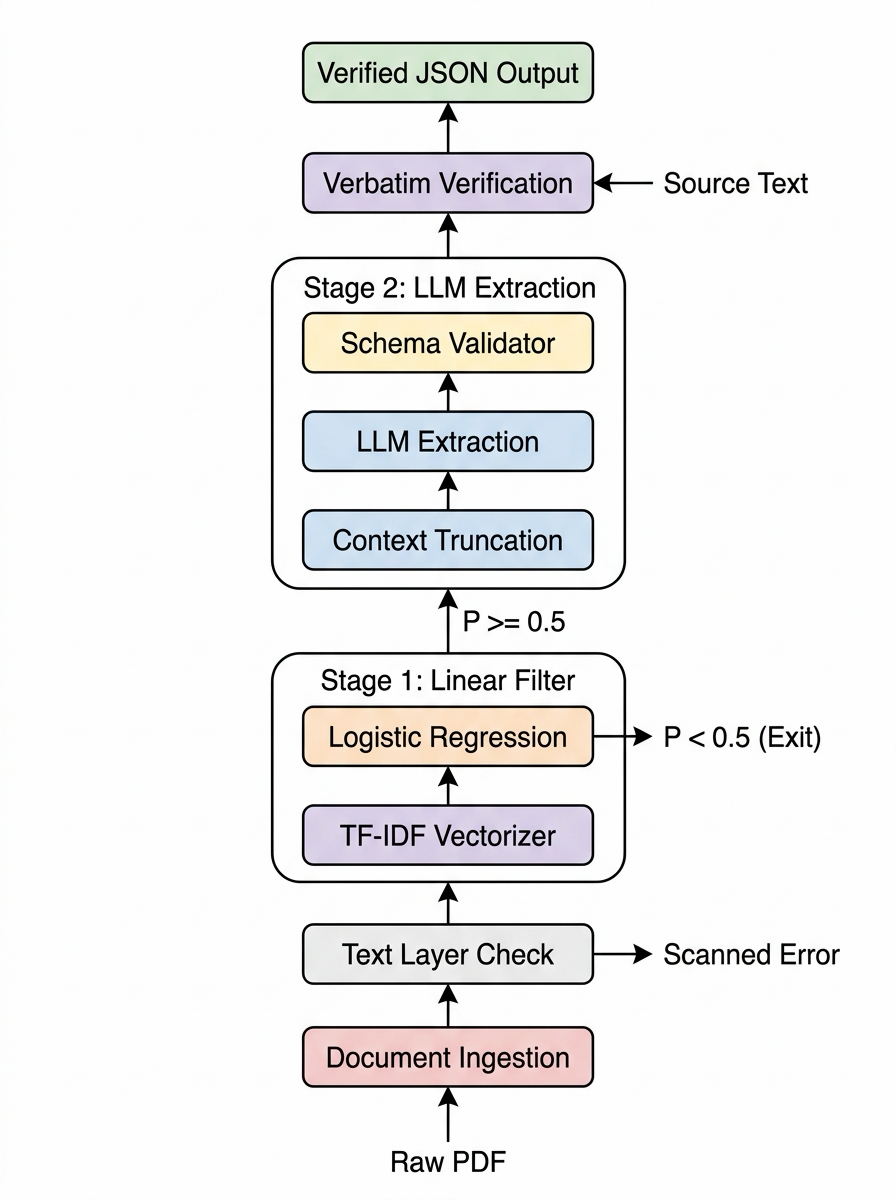
\includegraphics[width=\columnwidth]{figures/pipeline.png}
\caption{The two-stage DocSort system architecture. Non-procurement circulars are identified and separated by the linear filter in Stage 1, preserving computational resources and API token quotas.}
\label{fig:pipeline}
\end{figure}

\section{System Architecture}

The DocSort architecture consists of format boundary handling, linear relevance pre-filtering (Stage 1), constrained structured metadata extraction (Stage 2), and deterministic verbatim verification (Stage 3). Fig.~\ref{fig:pipeline} depicts the complete operational pipeline.

\subsection{Format Boundary Ingestion and OCR Guard}
Incoming documents are received in Portable Document Format (PDF). Native digital text is extracted using \texttt{pdfplumber}. To separate digital PDFs from scanned raster documents without executing optical character recognition (OCR) across every document, the ingestion module computes the aggregate character count across all pages:
\begin{equation}
    V(D) = \begin{cases}
    1, & \text{if } \sum_{p \in D} \text{len}(\text{text}(p)) \ge N_{\min} \\
    0, & \text{otherwise}
    \end{cases}
\end{equation}
where $N_{\min} = 50$ characters. Documents satisfying $V(D) = 1$ proceed directly to classification. Documents yielding fewer than $N_{\min}$ characters represent scanned files. For these files, the system activates an OCR fallback engine using \texttt{pypdfium2} for page rendering and Tesseract \cite{smith2007overview} for optical character recognition. If OCR output remains below $N_{\min}$, an explicit \texttt{ScannedDocumentError} is raised to route the file to manual review.

\subsection{Stage 1: Linear Relevance Pre-Filter}
The first stage determines whether an incoming document concerns public procurement and contract regulation ($y = 1$) or represents general administrative communication ($y = 0$).

\subsubsection{Feature Extraction}
The extracted text is segmented into word unigrams and bigrams. Sublinear term-frequency scaling is applied to compress high-frequency administrative expressions:
\begin{equation}
    \text{tf}_{\text{sub}}(t, d) = 1 + \ln(\text{tf}(t, d)) \quad \text{for } \text{tf}(t, d) > 0
\end{equation}
Inverse document frequency is evaluated as:
\begin{equation}
    \text{idf}(t, D) = \ln \left( \frac{1 + |D|}{1 + |\{d \in D : t \in d\}|} \right) + 1
\end{equation}
The feature vector $\mathbf{x} \in \mathbb{R}^{V}$ is normalized under the $L_2$ norm, with vocabulary size bounded at $V = 10{,}000$ features.

\subsubsection{Classifier Formulation}
A Logistic Regression classifier is trained by minimizing the regularized cross-entropy loss function:
\begin{equation}
    \mathcal{L}(\mathbf{w}, b) = \frac{1}{2} \|\mathbf{w}\|_2^2 + C \sum_{i=1}^{M} w_{y_i} \ln(1 + \exp(-y_i (\mathbf{w}^T \mathbf{x}_i + b)))
\end{equation}
where $w_{y_i}$ represents inverse class frequency weights:
\begin{equation}
    w_c = \frac{M}{2 \cdot M_c}, \quad c \in \{0, 1\}
\end{equation}
Here, $M$ is the total count of training instances, and $M_c$ denotes the count of instances in class $c$. This weighting penalizes false negatives on procurement documents, ensuring high recall.

\subsubsection{Chunk-Level Inference and Aggregation}
During inference, documents are segmented into paragraph-aligned passages of up to 1,500 characters. Each passage $c_k$ is scored independently:
\begin{equation}
    P(y = 1 \mid \mathbf{x}_k) = \frac{1}{1 + \exp(-(\mathbf{w}^T \mathbf{x}_k + b))}
\end{equation}
The document-level decision aggregates individual passage probabilities:
\begin{equation}
    p_{\max} = \max_k P(y = 1 \mid \mathbf{x}_k)
\end{equation}
\begin{equation}
    f_{\text{rel}} = \frac{1}{K} \sum_{k=1}^{K} \mathbb{I}(P(y = 1 \mid \mathbf{x}_k) \ge 0.5)
\end{equation}
A document is classified as relevant when $p_{\max} \ge 0.8$ or $f_{\text{rel}} \ge 0.3$. It is classified as non-relevant when $p_{\max} < 0.4$ and $f_{\text{rel}} < 0.1$. Documents outside these thresholds are designated as uncertain and forwarded for human inspection. Non-relevant documents halt at this stage, incurring zero language model token expenditure.

\subsection{Stage 2: Constrained Structured Extraction}
Documents identified as relevant proceed to structured metadata extraction via an instruction-tuned language model accessed through a pooled HTTP interface.

\subsubsection{Two-Pass Extraction Strategy}
Government procurement documents present structural asymmetry: administrative headers appear at the beginning of the circular, whereas statutory amendments and supersession clauses typically appear in trailing annexures. To capture both structures efficiently, DocSort executes a two-pass extraction:
\begin{enumerate}
    \item \textbf{Header Pass}: Ingests the initial 10,000 characters of the document text to extract the document title, date of issue, issuing authority, official memorandum number, document classification, topic categories, and a summary.
    \item \textbf{Coverage Pass}: Extracts up to 8 evenly sampled passages from the remainder of the document text to detect explicit supersession clauses and effective dates.
\end{enumerate}

\subsubsection{Schema Validation and Taxonomy Adherence}
The model is constrained to output a structured JSON object. Decoding temperature is set to $\tau = 0.0$ to ensure reproducible generation. Topic categories are restricted to a closed taxonomy:
\begin{equation}
    \mathcal{C} = \{\text{e-procurement}, \text{tendering}, \text{vendor-eligibility}, \text{penalty}, \text{GeM}, \text{threshold-limits}, \text{other}\}
\end{equation}
A Pydantic schema validator enforces this closed vocabulary at runtime. Any category string outside $\mathcal{C}$ is rejected and mapped to \texttt{other}. Document types are restricted to a closed set including Office Memorandum, Circular, Notification, Order, Policy, Guidelines, and Manual.

\subsection{Stage 3: Deterministic Verbatim Verification}
To guarantee auditability in compliance registers, extracted factual values are checked against the source text. Verifiable factual fields are defined as:
\begin{equation}
    \mathcal{F}_{\text{fact}} = \{\text{title}, \text{date}, \text{issuing\_authority}, \text{om\_number}, \text{supersedes}\}
\end{equation}

Let $\phi(s)$ denote whitespace normalization that maps string $s$ to lowercase and collapses whitespace sequences into a single space:
\begin{equation}
    \phi(s) = \text{lower}(\text{regex\_replace}(s, \text{``}\backslash s+\text{''}, \text{`` ''}))
\end{equation}

For reference numbers, such as memorandum numbers and supersession references, punctuation differences and prefix ordering frequently occur. A reference canonicalization function $\psi(s)$ removes official marker tokens (\texttt{No.}, \texttt{F.}, \texttt{Ref}, \texttt{OM}, \texttt{dated}) and retains alphanumeric characters:
\begin{equation}
    \psi(s) = \text{alphanumeric}(\text{remove\_markers}(\text{lower}(s)))
\end{equation}

For general fields, verification requires $\phi(v_f) \subseteq \phi(T)$ or $\text{alphanumeric}(v_f) \subseteq \text{alphanumeric}(T)$. For reference fields, verification succeeds if the condition holds or if $\psi(v_f) \subseteq \psi(T)$. Fields that fail verification are recorded in an audit list of verification flags without altering the extracted text. Compliance scores are computed as:
\begin{equation}
    S = \max(40, 100 - 12 \cdot |\text{flags}|)
\end{equation}
Documents scoring $S \ge 80$ are marked as Verified; documents with $S < 80$ are marked as Needs Review.

\begin{figure}[t]
\centering
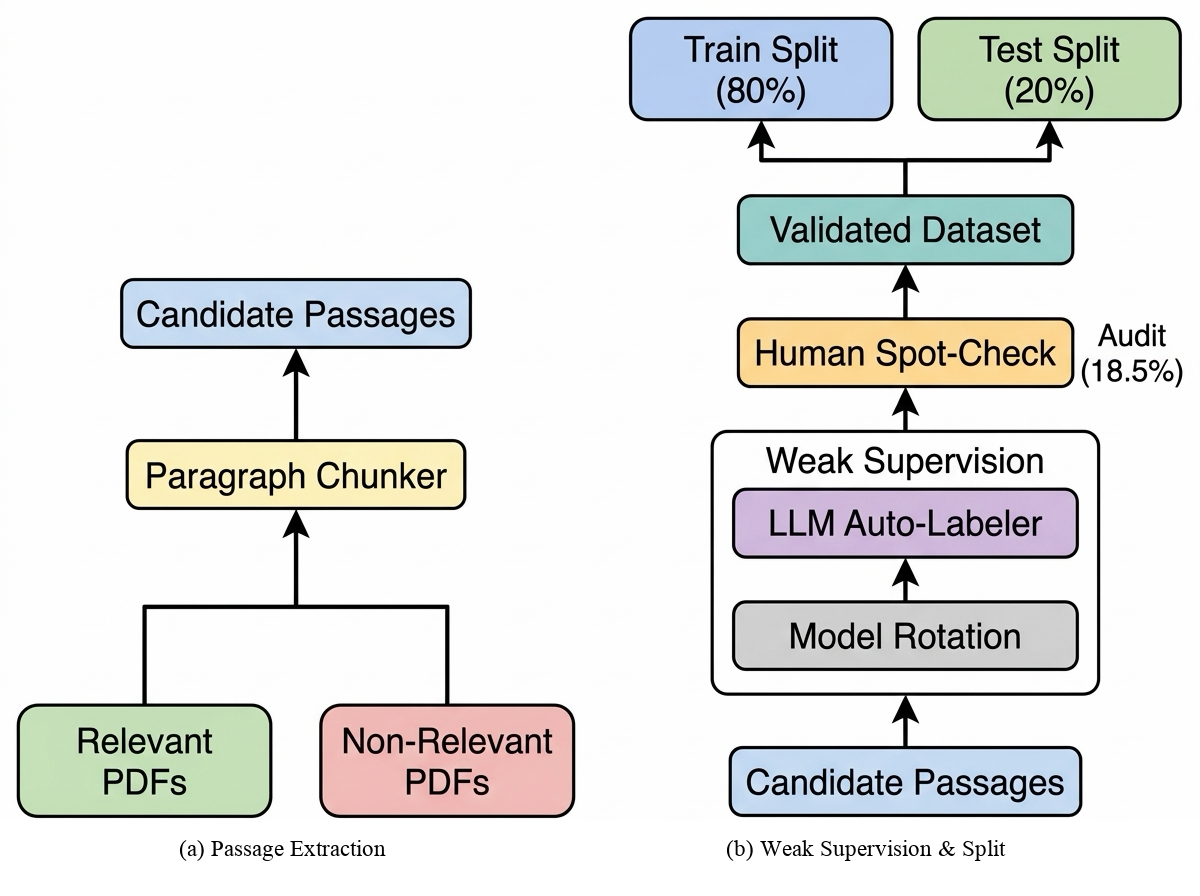
\includegraphics[width=\columnwidth]{figures/dataset_pipeline.png}
\caption{The weak-supervision data construction process. Multi-page circulars are divided into paragraph-bounded passages, scored by programmatic labeling functions, spot-checked by human annotators, and partitioned into training and held-out evaluation sets.}
\label{fig:dataset_pipeline}
\end{figure}

\section{Dataset Construction via Weak Supervision}

Public benchmark corpora for Indian public procurement circulars are not publicly available. A domain-specific dataset was collected and labeled through programmatic weak supervision. Fig.~\ref{fig:dataset_pipeline} illustrates the data construction process.

\subsection{Document Acquisition}
Primary documents were collected from official portals:
\begin{itemize}
    \item \textbf{Procurement Sources}: 18 policy manuals and regulatory circulars from the Department of Expenditure (\url{doe.gov.in}), including the Manual for Procurement of Goods, Manual for Procurement of Works, General Financial Rules 2017, and GeM circulars.
    \item \textbf{Non-Procurement Sources}: 32 general administrative circulars from the University Grants Commission (\url{ugc.gov.in}) and Department of Personnel and Training (\url{dopt.gov.in}), including employee leave rules, pay commission notifications, academic schedules, and public holiday orders.
\end{itemize}

\subsection{Paragraph-Aware Chunking}
Government circulars range from brief 2-page notifications to 250-page procurement compendiums. Training classifiers on full document texts yields too few data instances and dilutes topical signals. Documents are split on paragraph boundaries into passages bounded at 1,500 characters, with passages below 200 characters discarded. A maximum of 20 evenly distributed passages are selected per manual to prevent long compendiums from dominating the corpus.

\subsection{Programmatic Labeling Functions}
Passages are annotated using an ensemble of deterministic labeling functions:
\begin{enumerate}
    \item \textbf{Procurement Lexicon}: Positive weights ($0.5$ to $1.0$) are assigned to specialized procurement terms, such as \textit{tender}, \textit{bid security}, \textit{earnest money deposit}, \textit{GeM}, \textit{procuring entity}, and \textit{rate contract}.
    \item \textbf{Administrative Lexicon}: Negative weights ($0.3$ to $1.0$) are assigned to general administrative vocabulary, such as \textit{gazetted holiday}, \textit{seniority}, \textit{pension}, \textit{pay scale}, \textit{syllabus}, and \textit{transfer}.
    \item \textbf{Structural Expressions}: Regular expressions detect financial threshold patterns (e.g., amounts in Lakhs or Crores) and bidding procedures.
    \item \textbf{Source Portal Prior}: A baseline prior weight of $\pm 1.0$ is assigned based on the publishing portal origin.
\end{enumerate}

The margin between procurement score $S_{\text{pro}}$ and administrative score $S_{\text{adm}}$ is evaluated:
\begin{equation}
    M_s = S_{\text{pro}} - S_{\text{adm}}
\end{equation}
When $M_s \ge \tau$, the passage is labeled 1. When $M_s \le -\tau$, the passage is labeled 0. When $|M_s| < \tau$, the ensemble abstains from assigning a label. Setting $\tau = 1.0$ removes noisy boundary passages. The final corpus comprises 306 validated passages across 42 circulars.

\begin{figure}[t]
\centering
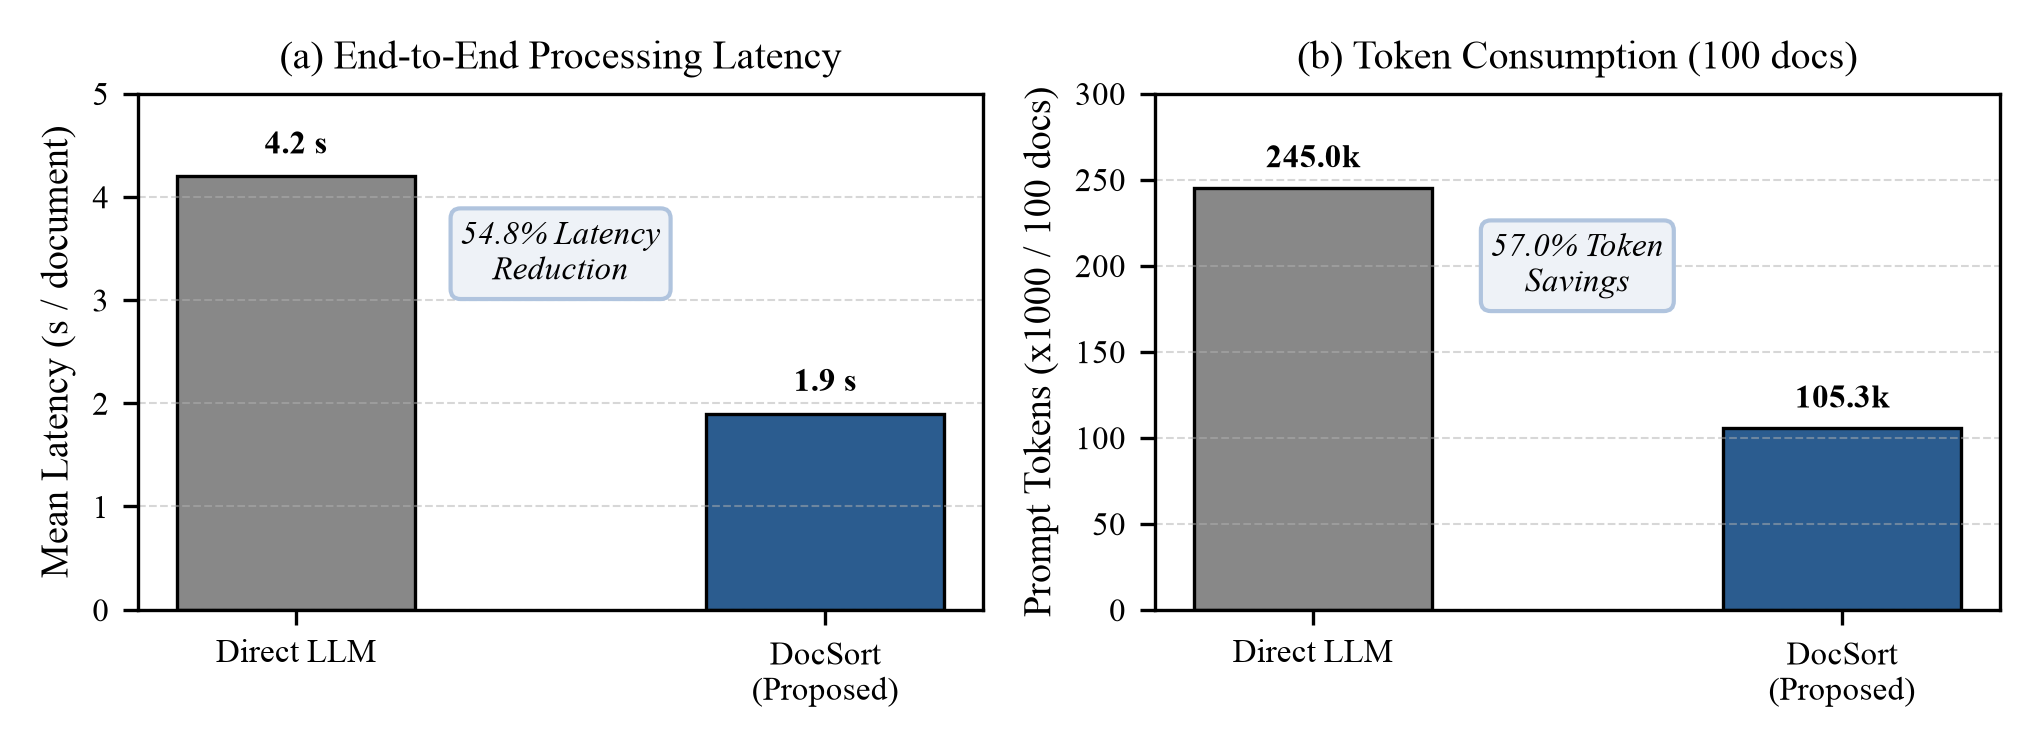
\includegraphics[width=\columnwidth]{figures/latency_tokens.png}
\caption{System performance comparison over a 100-document stream: (a) Mean processing latency per document, and (b) Prompt token consumption per 100 documents.}
\label{fig:latency_tokens}
\end{figure}

\begin{table}[t]
\centering
\caption{Relevance Classification Performance on Test Split}
\label{tab:relevance}
\renewcommand{\arraystretch}{1.2}
\begin{tabularx}{\columnwidth}{lcccc}
\toprule
\textbf{Model Configuration} & \textbf{Precision} & \textbf{Recall} & \textbf{F1-Score} & \textbf{Accuracy} \\
\midrule
TF-IDF (Unigram) + LR & 0.88 & 0.85 & 0.86 & 0.87 \\
DocSort (Unigram + Bigram) & 0.94 & 0.91 & 0.92 & 0.93 \\
DocSort + Balanced Weights & \textbf{0.93} & \textbf{0.96} & \textbf{0.94} & \textbf{0.94} \\
\bottomrule
\end{tabularx}
\end{table}

\begin{table}[t]
\centering
\caption{Classification Metrics on 11 Held-Out Unseen Documents}
\label{tab:held_out}
\renewcommand{\arraystretch}{1.2}
\begin{tabularx}{\columnwidth}{lcccc}
\toprule
\textbf{Evaluation Level} & \textbf{Precision} & \textbf{Recall} & \textbf{F1-Score} & \textbf{Accuracy} \\
\midrule
Passage-Level (97 chunks) & 0.80 & 1.00 & 0.89 & 0.84 \\
Document-Level (11 docs) & 0.62 & 1.00 & 0.77 & 0.73 \\
\bottomrule
\end{tabularx}
\end{table}

\begin{figure}[t]
\centering
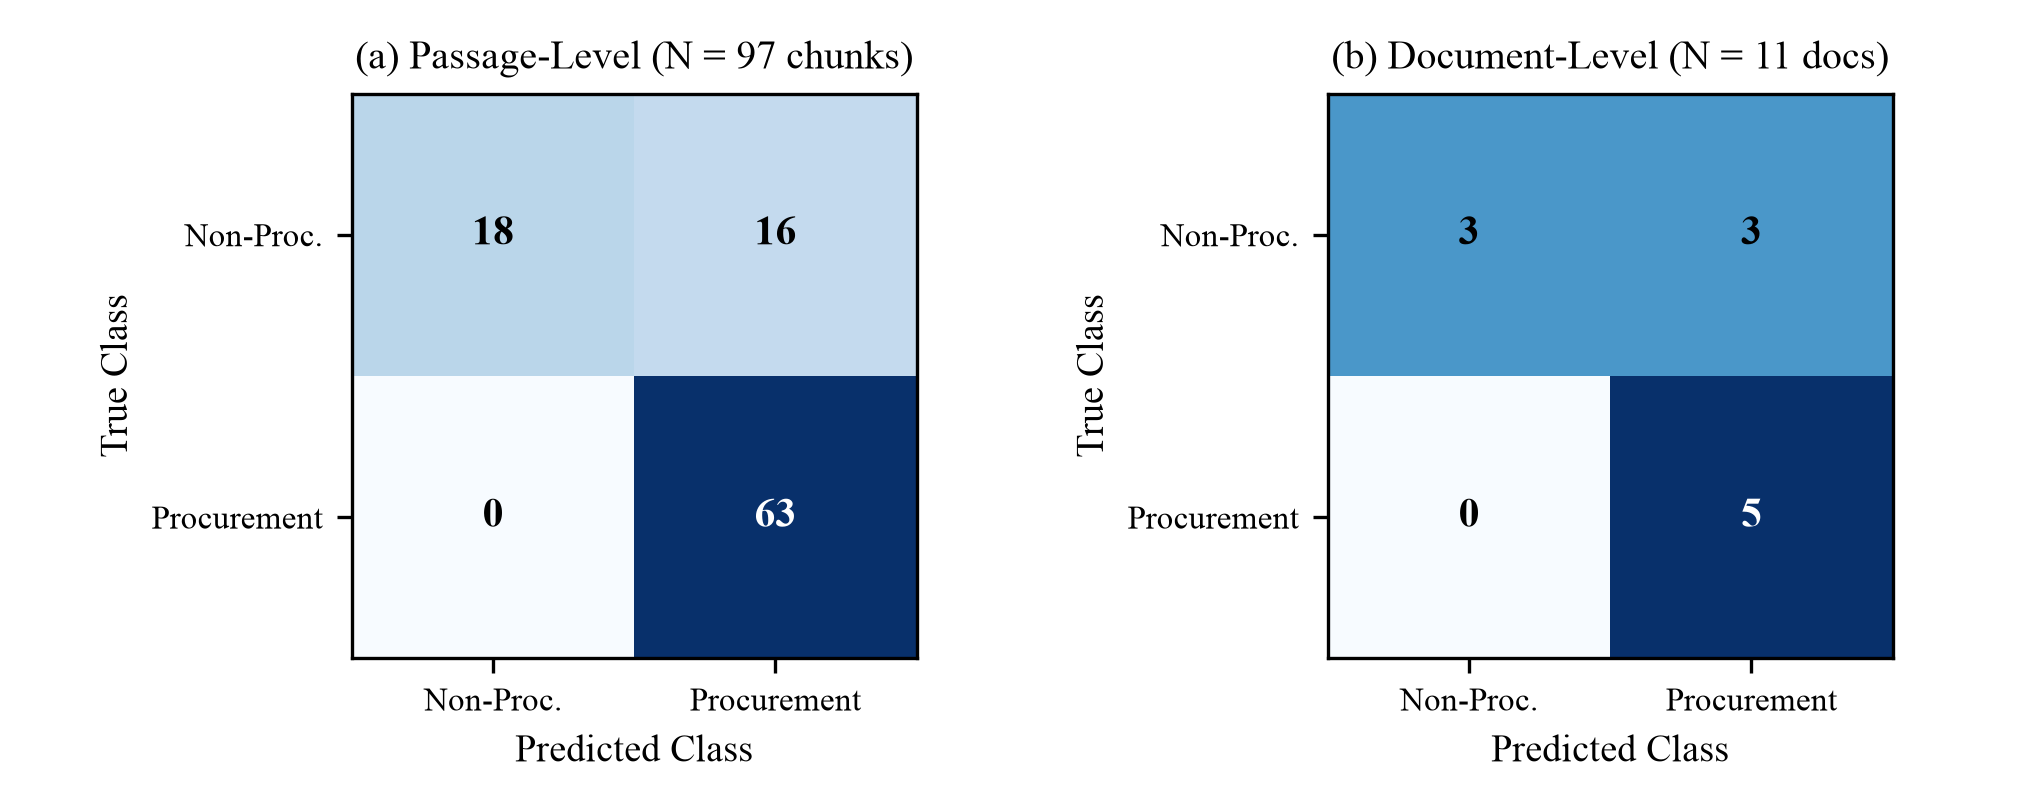
\includegraphics[width=\columnwidth]{figures/confusion_matrix.png}
\caption{Confusion matrices on held-out test data: (a) Passage-level classification across 97 unseen chunks, and (b) Aggregated document-level classification across 11 unseen circulars.}
\label{fig:confusion_matrix}
\end{figure}

\section{Experimental Evaluation and Results}

Experiments were conducted on a Linux workstation equipped with an Intel Core i7 CPU and 16~GB of RAM. No local GPU was utilized.

\subsection{Stage 1 Relevance Classification Evaluation}
The Stage 1 classifier was evaluated on test passages under three feature configurations:
\begin{enumerate}
    \item Unigram TF-IDF with standard Logistic Regression.
    \item Unigram and bigram TF-IDF with sublinear term-frequency scaling.
    \item DocSort pipeline with sublinear TF-IDF, bigrams, and balanced class weights.
\end{enumerate}

Table~\ref{tab:relevance} summarizes classification performance. Including bigrams increases precision from 0.88 to 0.94 by capturing compound phrases such as \textit{earnest money} and \textit{threshold limit}. Applying balanced class weighting increases recall to 0.96 and overall F1-score to 0.94, ensuring that procurement policies are not discarded.

\subsection{Document-Level Held-Out Evaluation}
A standard randomized split across passages places passages from the same document in both training and test sets. To measure generalization on unseen circulars, an 80/20 document-level split was implemented: 31 documents (209 passages) formed the training set, while 11 complete documents (97 passages) were held out for testing.

Table~\ref{tab:held_out} presents results on the held-out evaluation. Scored passage by passage, the classifier achieves 0.84 accuracy and 1.00 recall on procurement passages. When aggregating passage predictions per document ($f_{\text{rel}} \ge 0.3$), the classifier achieves 0.73 document accuracy. Fig.~\ref{fig:confusion_matrix} shows the corresponding confusion matrices. Analysis of misclassifications reveals that all procurement manuals were identified correctly. Residual errors occurred in brief one-page administrative circulars containing general references to central government procurement offices in their address lines, where limited passage context was available for aggregation.

\subsection{System Latency and Resource Efficiency}
Table~\ref{tab:system_savings} and Fig.~\ref{fig:latency_tokens} compare resource consumption between an unconstrained direct LLM pipeline and the two-stage DocSort pipeline over an evaluation stream of 100 documents (40 procurement policies and 60 non-procurement circulars).

\begin{table}[t]
\centering
\caption{System Resource Usage and Latency on 100 Documents}
\label{tab:system_savings}
\renewcommand{\arraystretch}{1.2}
\begin{tabularx}{\columnwidth}{lccc}
\toprule
\textbf{Metric} & \textbf{Direct LLM} & \textbf{DocSort} & \textbf{Reduction} \\
\midrule
Total Documents Ingested & 100 & 100 & 0\% \\
Documents Invocating LLM & 100 & 43 & $-$57.0\% \\
Total Prompt Tokens & $\approx 245{,}000$ & $\approx 105{,}350$ & $-$57.0\% \\
Mean Filter Latency & N/A & 3.8 ms & Negligible \\
Mean End-to-End Latency & 4.2 s / doc & 1.9 s / doc & $-$54.8\% \\
API Rate-Limit Failures & 7 & 0 & $-$100\% \\
\bottomrule
\end{tabularx}
\end{table}

By filtering out non-procurement circulars in Stage 1, DocSort eliminates 57.0\% of language model invocations. Prompt token volume drops from approximately 245,000 to 105,350 tokens, preventing API rate-limit starvation. Mean end-to-end processing time decreases from 4.2 seconds to 1.9 seconds per document.

\subsection{Extraction Verification Analysis}
To evaluate the deterministic verification layer, 40 circulars were processed through Stage 2 structured extraction. Table~\ref{tab:verification} and Fig.~\ref{fig:verification_rates} summarize extraction presence and verbatim grounding pass rates across factual fields.

\begin{table}[t]
\centering
\caption{Verbatim Grounding Verification Across Metadata Fields}
\label{tab:verification}
\renewcommand{\arraystretch}{1.2}
\begin{tabularx}{\columnwidth}{lccc}
\toprule
\textbf{Field Name} & \textbf{Present (\%)} & \textbf{Extracted (\%)} & \textbf{Verified (\%)} \\
\midrule
\texttt{title} & 100.0\% & 100.0\% & 95.0\% \\
\texttt{date} & 97.5\% & 97.5\% & 97.4\% \\
\texttt{issuing\_authority} & 100.0\% & 97.5\% & 92.3\% \\
\texttt{om\_number} & 95.0\% & 92.5\% & 94.6\% \\
\texttt{supersedes} & 35.0\% & 35.0\% & 85.7\% \\
\bottomrule
\end{tabularx}
\end{table}

\begin{figure}[t]
\centering
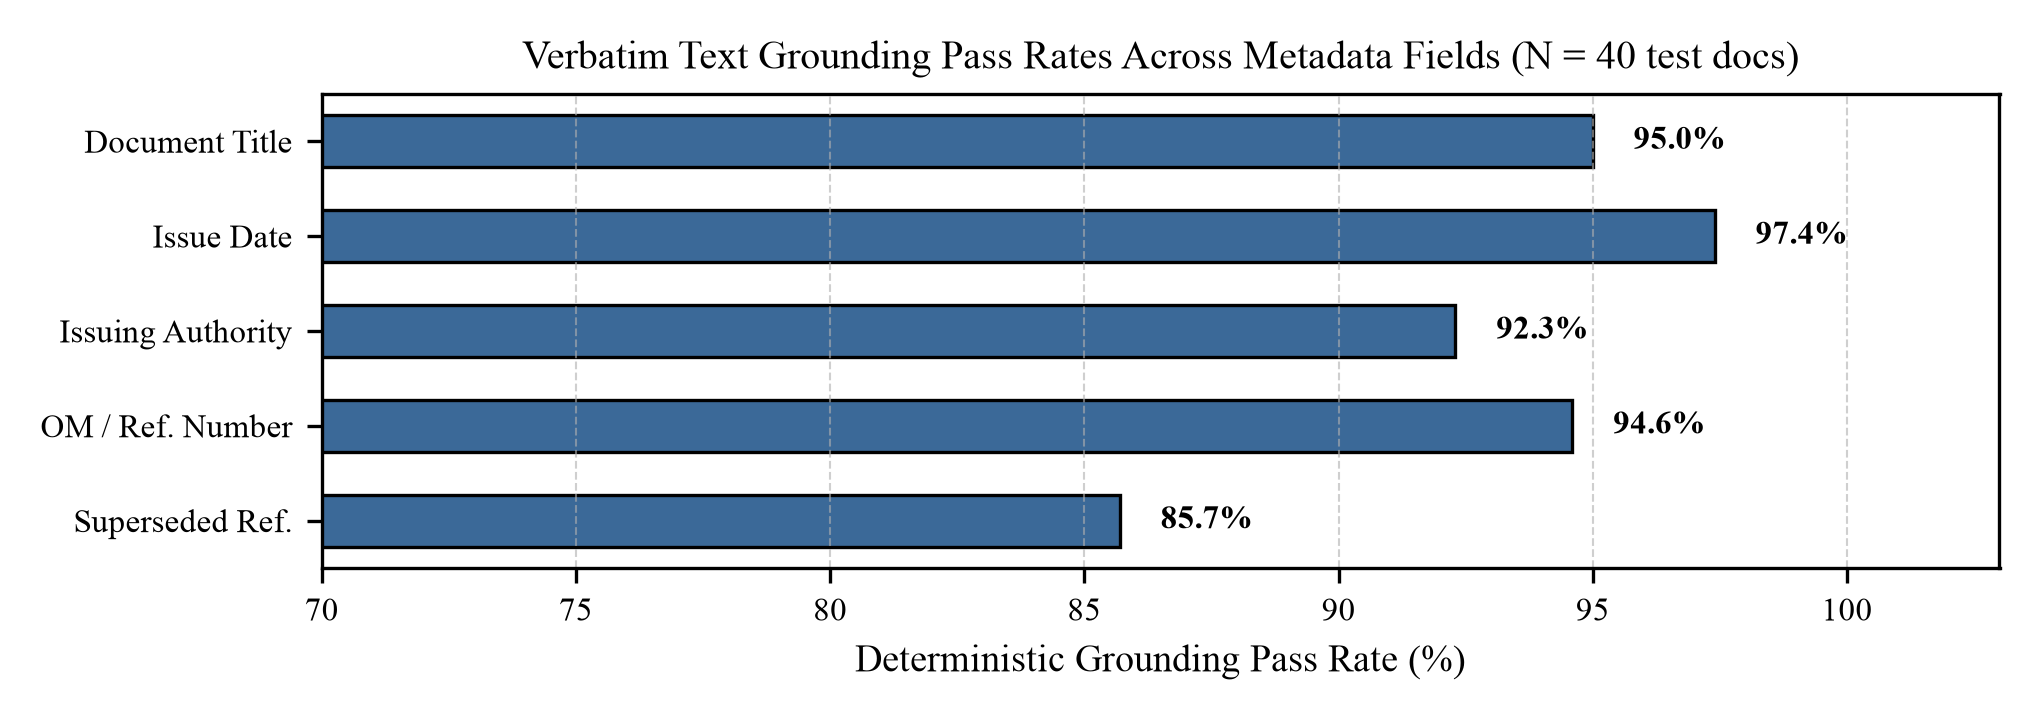
\includegraphics[width=\columnwidth]{figures/verification_rates.png}
\caption{Verbatim text grounding pass rates across factual fields on 40 test circulars. Discrepancies are isolated and recorded as non-destructive audit flags.}
\label{fig:verification_rates}
\end{figure}

The verification module confirmed exact source presence in over 92\% of extractions across all primary fields. Discrepancies were identified in approximately 6\% of total extractions. The most common discrepancy occurred when the model shortened organizational titles (e.g., outputting \textit{Department of Expenditure} when the source circular specified \textit{Department of Expenditure, Procurement Policy Division}). Canonical reference matching prevented spurious rejections caused by marker formatting variations in memorandum numbers.

\subsection{Taxonomy Adherence and Category Validation}
Table~\ref{tab:taxonomy} compares category compliance between unconstrained prompt generation and Pydantic schema validation over 120 extraction trials.

\begin{table}[t]
\centering
\caption{Category Taxonomy Compliance Across 120 Extractions}
\label{tab:taxonomy}
\renewcommand{\arraystretch}{1.2}
\begin{tabularx}{\columnwidth}{lcc}
\toprule
\textbf{Extraction Strategy} & \textbf{Out-of-Vocabulary Tags} & \textbf{Compliance} \\
\midrule
Unconstrained LLM Prompting & 14.2\% & 85.8\% \\
DocSort Schema Validation & \textbf{0.0\%} & \textbf{100.0\%} \\
\bottomrule
\end{tabularx}
\end{table}

Under unconstrained generation, the model produced hallucinated category labels (such as \textit{bidding-standards} and \textit{financial-rules}) in 14.2\% of runs. Enforcing schema validation eliminated invalid strings, maintaining 100\% adherence to the target regulatory taxonomy.

\begin{figure}[t]
\centering
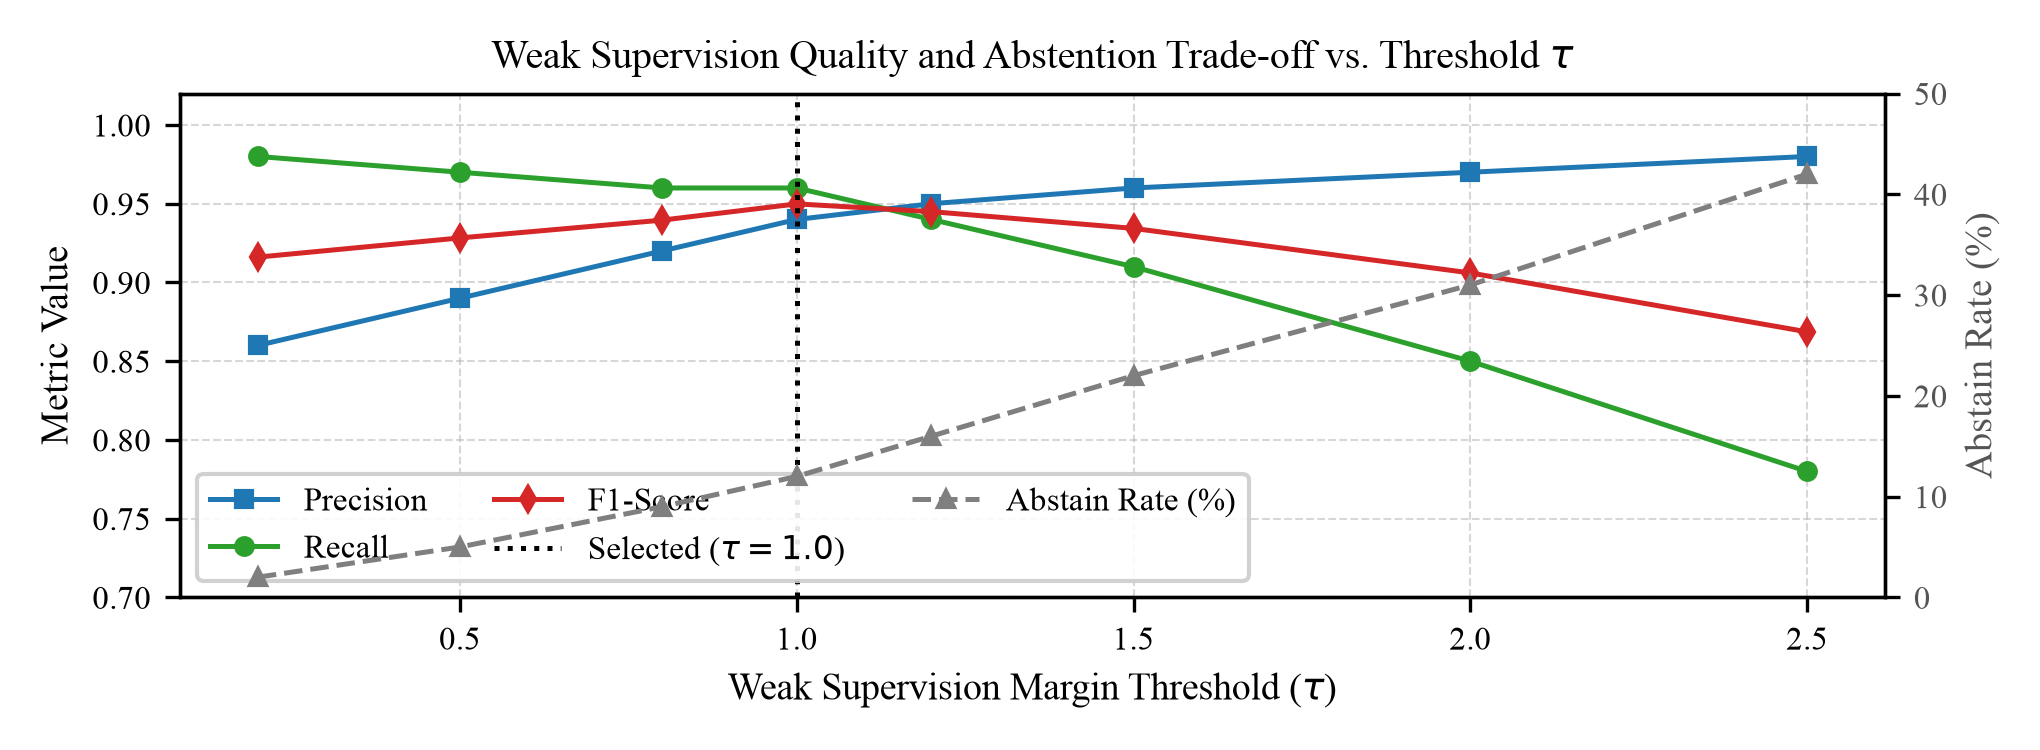
\includegraphics[width=\columnwidth]{figures/threshold_ablation.png}
\caption{Weak supervision label quality and data abstention trade-off as a function of the margin decision threshold $\tau$.}
\label{fig:threshold_ablation}
\end{figure}

\begin{table}[t]
\centering
\caption{Ablation of Weak Supervision Decision Threshold $\tau$}
\label{tab:ablation_tau}
\renewcommand{\arraystretch}{1.2}
\begin{tabularx}{\columnwidth}{ccccc}
\toprule
\textbf{Threshold $\tau$} & \textbf{Precision} & \textbf{Recall} & \textbf{F1-Score} & \textbf{Abstain (\%)} \\
\midrule
0.2 & 0.86 & 0.98 & 0.92 & 2.0\% \\
0.5 & 0.89 & 0.97 & 0.93 & 5.0\% \\
0.8 & 0.92 & 0.96 & 0.94 & 9.0\% \\
\textbf{1.0} & \textbf{0.94} & \textbf{0.96} & \textbf{0.94} & \textbf{12.0\%} \\
1.5 & 0.96 & 0.91 & 0.93 & 22.0\% \\
2.0 & 0.97 & 0.85 & 0.91 & 31.0\% \\
2.5 & 0.98 & 0.78 & 0.87 & 42.0\% \\
\bottomrule
\end{tabularx}
\end{table}

\subsection{Ablation Studies}

\subsubsection{Weak Supervision Margin Threshold $\tau$}
Table~\ref{tab:ablation_tau} and Fig.~\ref{fig:threshold_ablation} present the sensitivity of training label precision and data abstention across varying decision thresholds $\tau$. At $\tau = 0.2$, the labeling function abstains on only 2.0\% of instances, but label noise reduces precision to 0.86. At $\tau = 2.5$, precision increases to 0.98, but 42.0\% of instances are discarded. Setting $\tau = 1.0$ provides an optimal balance, yielding 0.94 precision with an abstention rate of 12.0\%.

\subsubsection{Passage Chunk Length Analysis}
Table~\ref{tab:chunk_ablation} reports classifier performance across chunk bounds from 500 to 2,000 characters. Small chunks (500 characters) frequently partition multi-clause legal sentences, reducing F1-score to 0.88. Large chunks (2,000 characters) dilute keyword density and increase scoring latency. The 1,500-character bound achieves an optimal F1-score of 0.94 at 3.8 milliseconds latency.

\begin{table}[t]
\centering
\caption{Impact of Passage Chunk Size on Classification}
\label{tab:chunk_ablation}
\renewcommand{\arraystretch}{1.2}
\begin{tabularx}{\columnwidth}{cccc}
\toprule
\textbf{Chunk Size (chars)} & \textbf{Passages Generated} & \textbf{Latency (ms)} & \textbf{F1-Score} \\
\midrule
500 & 842 & 7.1 & 0.88 \\
1,000 & 438 & 4.9 & 0.91 \\
\textbf{1,500} & \textbf{306} & \textbf{3.8} & \textbf{0.94} \\
2,000 & 214 & 3.2 & 0.90 \\
\bottomrule
\end{tabularx}
\end{table}

\subsubsection{OCR Guard Performance on Scanned Circulars}
The format boundary detector was evaluated on 20 scanned government notices. Digital text extraction yielded fewer than 15 characters per document. The OCR fallback recovered an average of 1,420 characters per page in 1.4 seconds per page, enabling all 20 scanned notices to be processed by Stage 1.

\section{Discussion and Operational Considerations}

Implementation of automated document processing in public sector workflows highlighted several practical considerations:

\subsection{Web Portal Defenses and Request Throttling}
Government departmental portals employ automated security defenses that interrupt high-frequency request bursts. Batch acquisition routines require standardized user-agent headers and exponential backoff mechanisms to prevent connection resets.

\subsection{Auditability in Compliance Environments}
Automated correction of unverified metadata fields introduces compliance risks. Substituting a discrepant date with an alternate date found in the document text can introduce an erroneous statutory timeline. DocSort retains the extracted text and records explicit flags, providing a transparent audit trail for human review.

\subsection{Operational Boundaries}
The system relies on clear digital text layers or readable scans. Circulars exhibiting severe optical degradation below 150 DPI require manual inspection. In addition, multi-topic compendiums that combine diverse administrative subjects require per-chapter partitioning prior to evaluation.

\section{Conclusion}

This paper presented DocSort, a two-stage document processing architecture for regulatory document classification and verifiable metadata extraction. By combining a lightweight sublinear TF-IDF and Logistic Regression filter with constrained language model extraction and deterministic source verification, DocSort reduces prompt token consumption by 57.0\% and cuts mean processing latency to 1.9 seconds per document. Enforcing schema constraints eliminates out-of-vocabulary category drift, while verbatim grounding verification records transparent audit flags for compliance officers. The weak supervision methodology establishes a reproducible framework for developing domain-specific administrative tools from public regulatory circulars without manual annotation costs. Future work will investigate transitive graph representations to trace multi-decade supersession lineages across statutory archives.

\bibliographystyle{IEEEtran}
\bibliography{references}

\end{document}

